\documentclass[11pt,a4paper]{article}
\usepackage[utf8]{inputenc}
\usepackage[T1]{fontenc}
\usepackage[brazilian]{babel}
\usepackage{graphicx}
\usepackage{booktabs}
\usepackage{hyperref}
\usepackage{amsmath}
\usepackage{float}
\usepackage{geometry}

\geometry{margin=2.5cm}

\title{EP3: Avaliação e Seleção de Modelos de Aprendizado de Máquina \\
\large MAC0460/MAC5832 — DCC / IME-USP}
\author{Leonardo Heidi Almeida Murakami \\
NUSP: 11260186 \\
Curso: Bacharelado em Ciência da Computação}
\date{1º Semestre de 2026}

\begin{document}

\maketitle

\begin{abstract}
Este relatório apresenta os resultados do EP3. O objetivo foi praticar a avaliação e seleção de modelos usando a biblioteca \texttt{scikit-learn} no dataset \textit{Digits}. Testamos os algoritmos SVM, Random Forest, $k$-NN e Árvore de Decisão. O melhor modelo foi o SVM com kernel RBF, que alcançou 98,15\% de acurácia no conjunto de teste.
\end{abstract}

\section{Introdução}
O objetivo deste trabalho é aprender a avaliar e escolher modelos de machine learning de forma correta, evitando estimativas erradas de desempenho. 

Usamos o dataset \textit{Digits}, que possui 1.797 imagens de dígitos manuscritos (de 0 a 9). Cada imagem tem tamanho $8 \times 8$ pixels, gerando 64 atributos (\textit{features}). Avaliamos quatro algoritmos no problema: SVM, Random Forest, $k$-NN e Árvore de Decisão.

\section{Metodologia}
O projeto seguiu os seguintes passos:

\begin{enumerate}
    \item \textbf{Visualização:} Plotamos uma amostra das imagens do dataset para entender os dados (Figura~\ref{fig:sample_digits}).
    \item \textbf{Divisão dos dados:} Separamos o dataset de forma estratificada (mantendo a proporção das classes) em 70\% para treino (1.257 amostras) e 30\% para teste (540 amostras). O conjunto de teste foi guardado e usado só no final.
    \item \textbf{Padronização:} Usamos o \texttt{StandardScaler} para deixar os atributos na mesma escala (média 0 e variância 1). O ajuste foi feito apenas com os dados de treino.
    \item \textbf{Modelo Base:} Treinamos um SVM linear padrão ($C=1.0$) para servir como primeira comparação (Figura~\ref{fig:confusion_matrix_linear_svm_default}).
    \item \textbf{Otimização (Grid Search):} Testamos o SVM com kernel RBF variando os parâmetros $C$ e $\gamma$ em duas etapas: uma busca grossa (\textit{coarse}) e depois um refino (\textit{fine}).
    \item \textbf{Comparação de Modelos:} Usamos validação cruzada estratificada com 5 dobras (5-fold CV) para comparar os quatro algoritmos e escolher o melhor com base na acurácia média de validação.
\end{enumerate}

\begin{figure}[H]
    \centering
    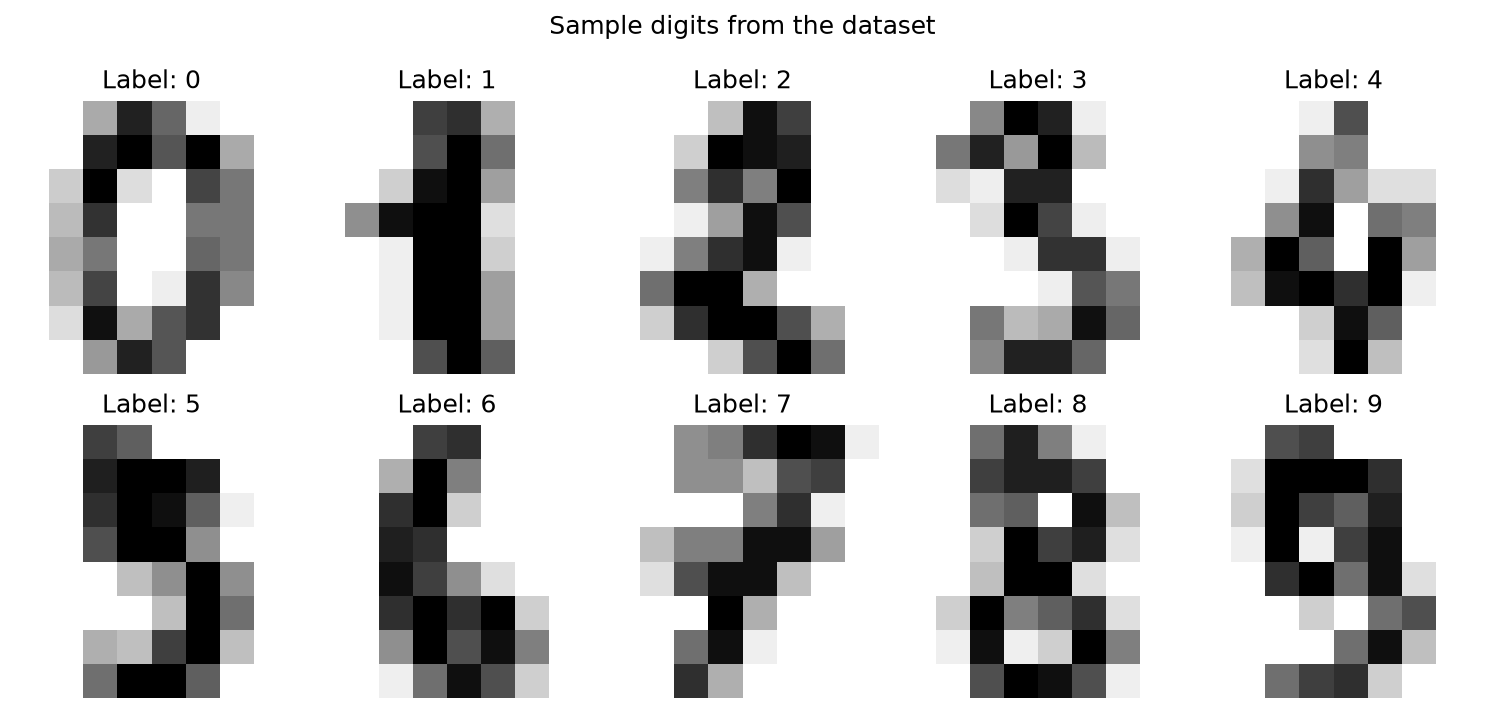
\includegraphics[width=0.5\textwidth]{images/sample_digits.png}
    \caption{Exemplos de dígitos do dataset Digits.}
    \label{fig:sample_digits}
\end{figure}

\begin{figure}[H]
    \centering
    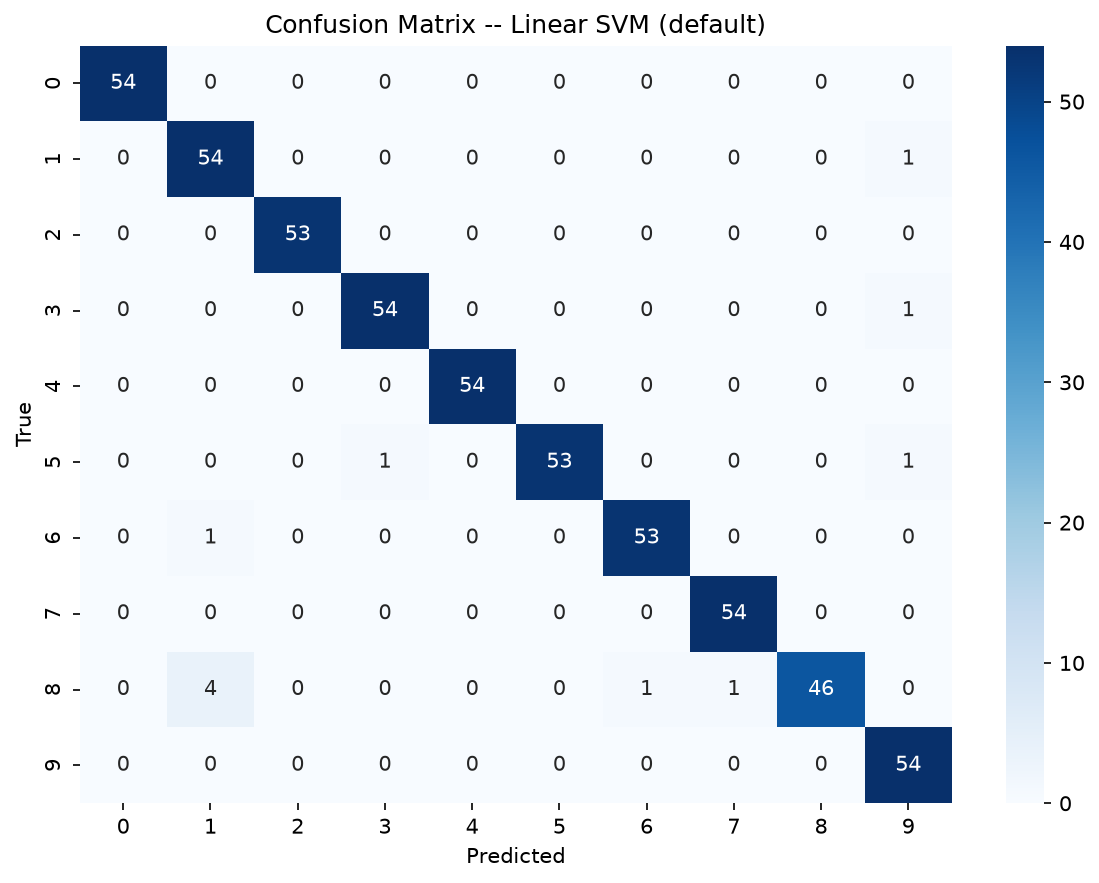
\includegraphics[width=0.45\textwidth]{images/confusion_matrix_linear_svm_default.png}
    \caption{Matriz de confusão do SVM linear com parâmetros padrão.}
    \label{fig:confusion_matrix_linear_svm_default}
\end{figure}

\section{Resultados}

\begin{itemize}
    \item \textbf{SVM Linear Padrão:} Alcançou acurácia de \textbf{97,96\%} no teste.
    \item \textbf{Grid Search Coarse:} Os melhores parâmetros foram $C=1.0$ e $\gamma=$\texttt{'scale'} (Validação: 98,17\%, Teste: 98,33\%).
    \item \textbf{Grid Search Fino:} Os parâmetros foram $C \approx 3.16$ e $\gamma=$\texttt{'auto'} (Validação: 98,17\%, Teste: 98,15\%).
\end{itemize}

A Tabela~\ref{tab:algorithm_comparison} mostra a comparação final entre todos os algoritmos testados com validação cruzada de 5 dobras. O gráfico correspondente está na Figura~\ref{fig:algorithm_comparison}.

\begin{table}[H]
\centering
\caption{Comparação de desempenho dos algoritmos.}
\label{tab:algorithm_comparison}
\begin{tabular}{lccc}
\toprule
\textbf{Algoritmo} & \textbf{Acurácia CV (Média)} & \textbf{Desvio Padrão CV} & \textbf{Acurácia Teste} \\
\midrule
SVM (RBF)     & 0,9801 & 0,0084 & 0,9815 \\
Random Forest & 0,9737 & 0,0054 & 0,9667 \\
$k$-NN        & 0,9682 & 0,0056 & 0,9722 \\
Árvore de Decisão  & 0,8497 & 0,0298 & 0,8574 \\
\bottomrule
\end{tabular}
\end{table}

\begin{figure}[H]
    \centering
    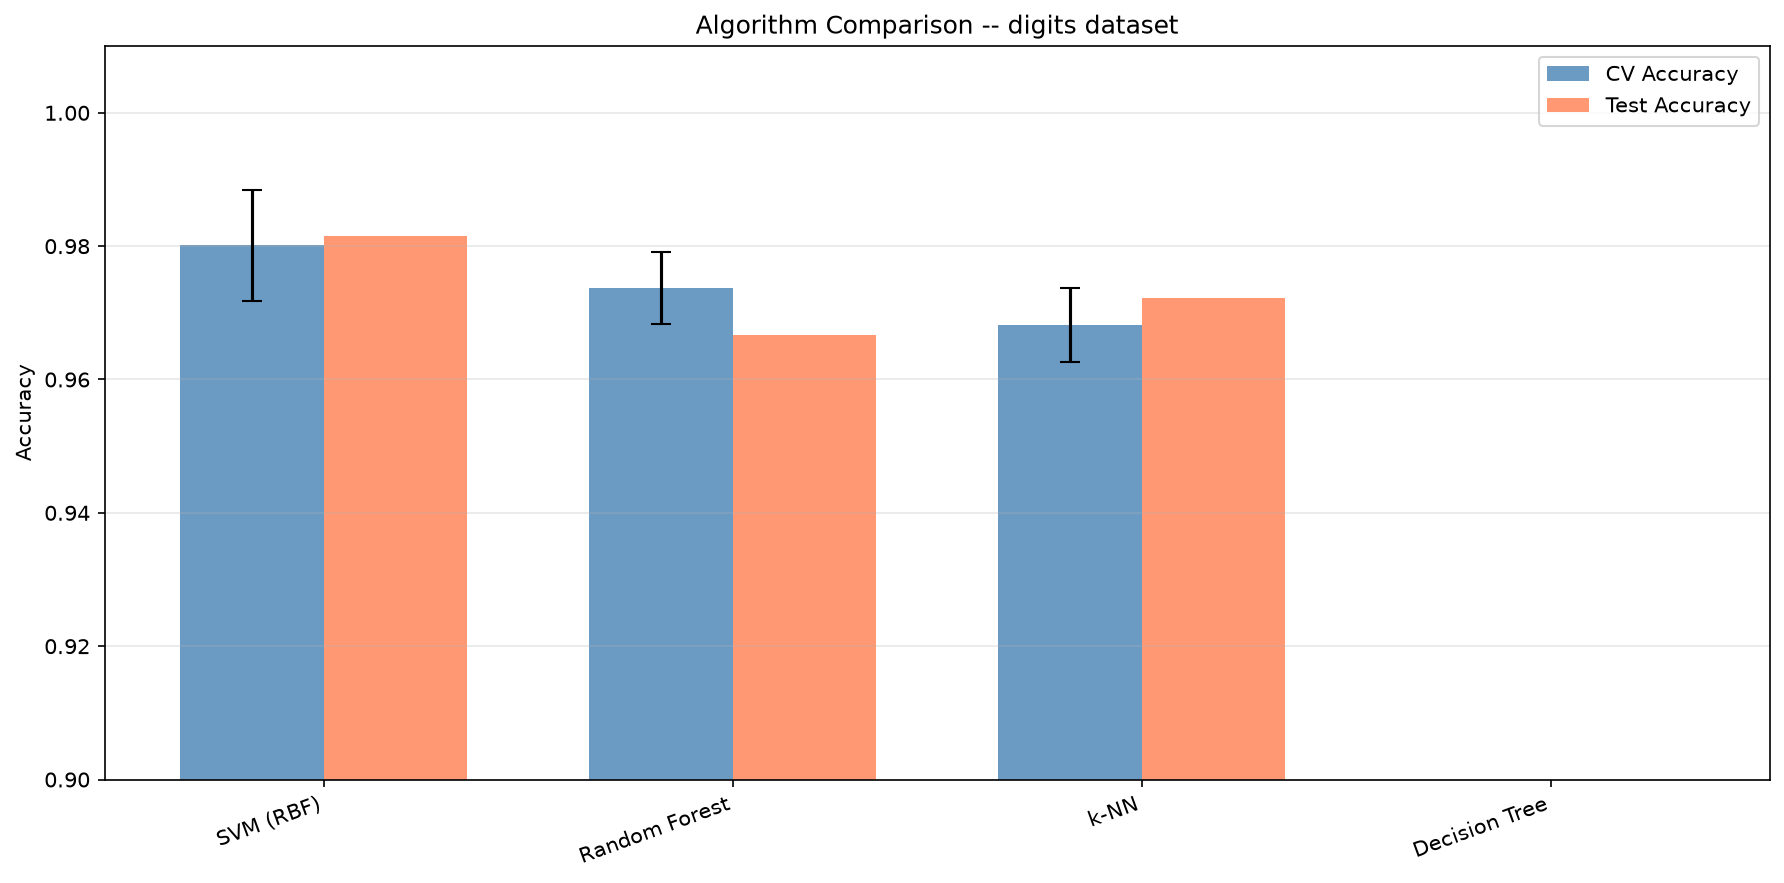
\includegraphics[width=0.5\textwidth]{images/algorithm_comparison.png}
    \caption{Acurácia de validação vs. teste por algoritmo.}
    \label{fig:algorithm_comparison}
\end{figure}

O melhor modelo final foi o \textbf{SVM (RBF)} com $C=10.0$ e $\gamma=0.01$. A Tabela~\ref{tab:classification_report} traz os detalhes de acertos por classe, e a Figura~\ref{fig:confusion_matrix_best_model} mostra sua matriz de confusão.

\begin{table}[H]
\centering
\caption{Relatório de classificação do melhor modelo SVM (RBF).}
\label{tab:classification_report}
\begin{tabular}{ccccc}
\toprule
\textbf{Classe (Dígito)} & \textbf{Precision} & \textbf{Recall} & \textbf{F1-Score} & \textbf{Support} \\
\midrule
0 & 1,00 & 1,00 & 1,00 & 54 \\
1 & 0,95 & 0,98 & 0,96 & 55 \\
2 & 1,00 & 0,98 & 0,99 & 53 \\
3 & 1,00 & 1,00 & 1,00 & 55 \\
4 & 0,95 & 0,98 & 0,96 & 54 \\
5 & 1,00 & 0,98 & 0,99 & 55 \\
6 & 0,98 & 1,00 & 0,99 & 54 \\
7 & 0,96 & 1,00 & 0,98 & 54 \\
8 & 1,00 & 0,92 & 0,96 & 52 \\
9 & 0,98 & 0,96 & 0,97 & 54 \\
\bottomrule
\end{tabular}
\end{table}

\begin{figure}[H]
    \centering
    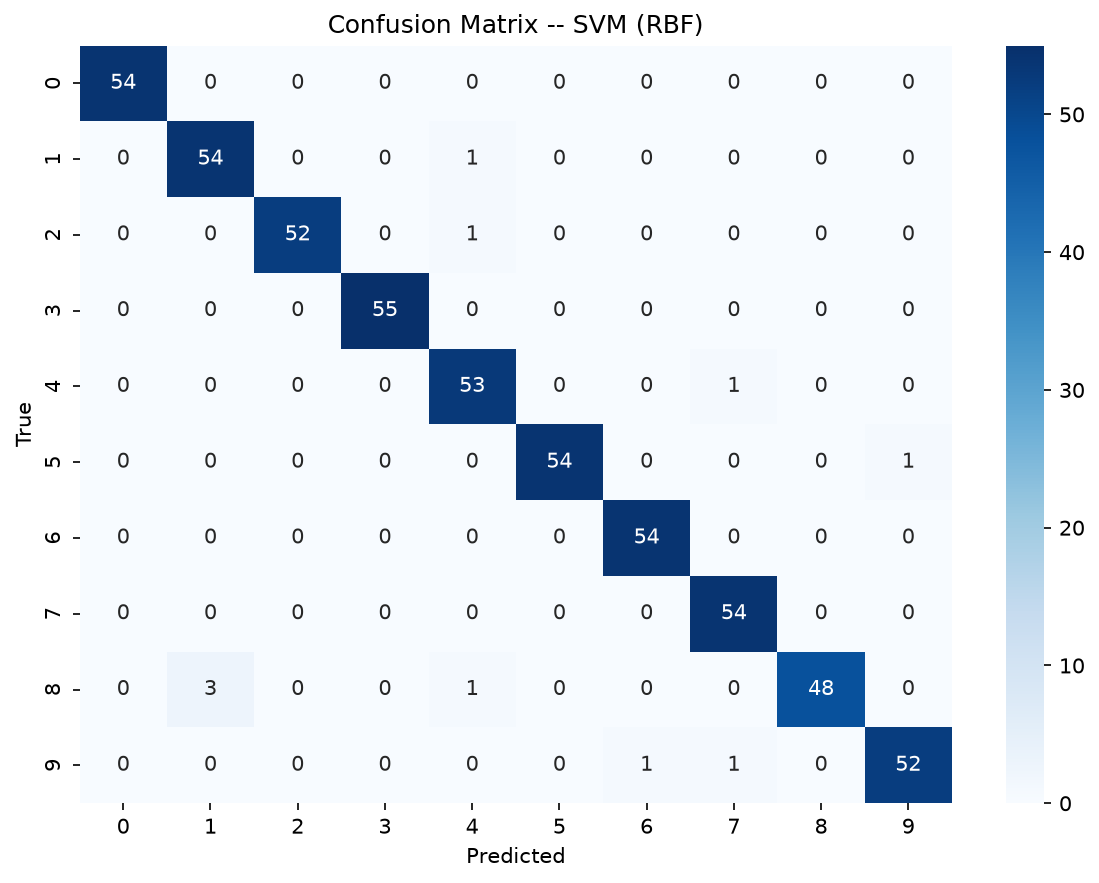
\includegraphics[width=0.45\textwidth]{images/confusion_matrix_best_model.png}
    \caption{Matriz de confusão do melhor modelo SVM RBF.}
    \label{fig:confusion_matrix_best_model}
\end{figure}

Separamos na Figura~\ref{fig:mispredicted_examples} os poucos exemplos que o modelo errou no conjunto de teste.

\begin{figure}[H]
    \centering
    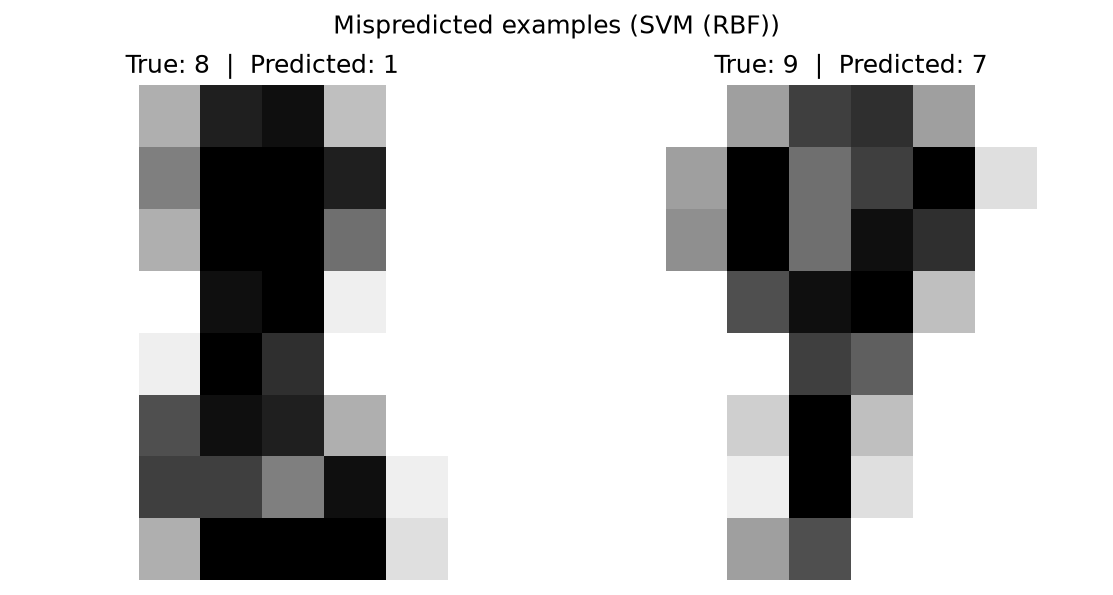
\includegraphics[width=0.45\textwidth]{images/mispredicted_examples.png}
    \caption{Exemplos de dígitos classificados incorretamente.}
    \label{fig:mispredicted_examples}
\end{figure}



\section{Conclusão}
O EP3 mostrou a importância de uma metodologia rígida. Separar um conjunto de teste isolado e usar a validação cruzada estratificada em 5 dobras nos deu a certeza de que os resultados são reais e confiáveis. O modelo SVM RBF se mostrou excelente para o reconhecimento dos dígitos manuscritos.

\section{Ferramentas de IA utilizadas}
Usamos ferramentas de IA de duas formas simples neste trabalho:
\begin{itemize}
    \item \textbf{No código:} Preenchimento automático (\textit{tab completion}) para acelerar a escrita de comandos do scikit-learn e estilização de gráficos.
    \item \textbf{No relatório:} Auxílio para organizar as tabelas e converter o texto resumido para a sintaxe correta do \LaTeX.
\end{itemize}
Toda a análise dos dados e escolhas de projeto foram feitas pelo próprio aluno.

\end{document}